\section{Eksperimentel Opstilling}
\begin{figure}[H]
    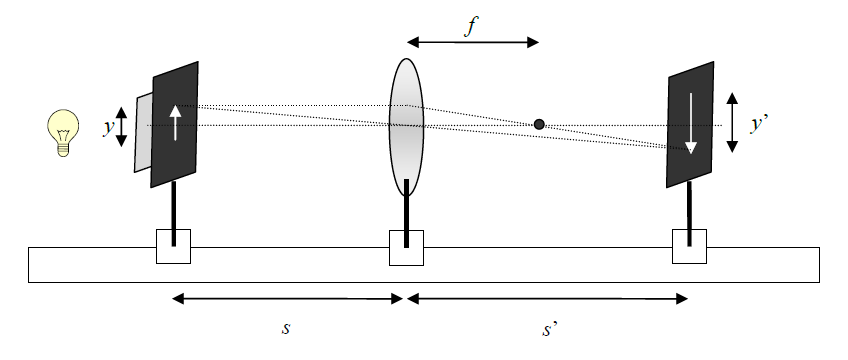
\includegraphics[width=\linewidth]{tegning.png}
    \caption{Billede af opstillingen. Alt opstillet på en optisk bænk. Fra venstre: En lyskilde, en maske, en linse  og til slut en skærm.}
    \label{fig:opstilling}
\end{figure}
På \cref{fig:opstilling}, ses et billede af opstillingen. Alle elementer monteres på en optisk bænk. I \forsogEt, anvdens en pære som lyskilde. Lyset føres igennem en maske, hvorpå der er en særk/diffusor anvendes. Til slut føres lyset igennem en linse, hvorpå det resulterende lys samles på en skærm. I \forsogTo, anvendes det omgivne lys som lyskilde. Masken er fjernet, og erstattet af endnu en linse. Denne gang observeres lyset blot direkte, ved at kigge igennem linserne, frem for at observere det på en skærm.
